\documentclass{article}
\usepackage{tikz}
\usetikzlibrary{positioning}

\begin{document}

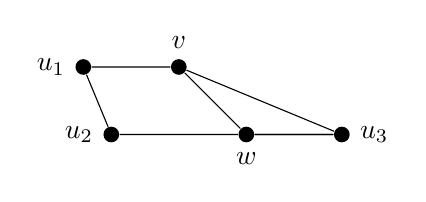
\begin{tikzpicture}[node distance=1cm]
    \node[circle,fill,inner sep=2pt,label=left:$u_1$] (u1) {};
    \node[circle,fill,inner sep=2pt,right=of u1,label=above:$v$] (v) {};
    \node[circle,fill,inner sep=2pt,below right=of v,label=below:$w$] (w) {};
    \node[circle,fill,inner sep=2pt,right=of w,label=right:$u_3$] (u3) {};
    \node[circle,fill,inner sep=2pt,below left=of v,label=left:$u_2$] (u2) {};

    \draw (u1) -- (v) -- (w) -- (u3) -- (v);
    \draw (u1) -- (u2) -- (w) -- (u3);
\end{tikzpicture}

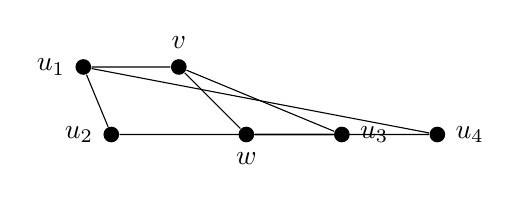
\begin{tikzpicture}[node distance=1cm]
    \node[circle,fill,inner sep=2pt,label=left:$u_1$] (u1) {};
    \node[circle,fill,inner sep=2pt,right=of u1,label=above:$v$] (v) {};
    \node[circle,fill,inner sep=2pt,below right=of v,label=below:$w$] (w) {};
    \node[circle,fill,inner sep=2pt,right=of w,label=right:$u_3$] (u3) {};
    \node[circle,fill,inner sep=2pt,right=of u3,label=right:$u_4$] (u4) {};
    \node[circle,fill,inner sep=2pt,below left=of v,label=left:$u_2$] (u2) {};

    \draw (u1) -- (v) -- (w) -- (u3) -- (v);
    \draw (u1) -- (u2) -- (w) -- (u3);
    \draw (u1) -- (u4) -- (w) -- (u3);
    \draw (u2) -- (u3);
\end{tikzpicture}

\end{document}